\documentclass[final,5p,times,twocolumn]{elsarticle}
\usepackage[T1]{fontenc}
\renewcommand{\ttdefault}{lmtt} % Embedded vector Latin Modern Typewriter
\usepackage{microtype,graphicx,booktabs,amsmath,amssymb,array,tabularx,longtable,xurl,placeins}
\usepackage[hypertexnames=false]{hyperref}
\setlength{\emergencystretch}{2em}
\renewcommand{\topfraction}{0.9}
\renewcommand{\bottomfraction}{0.8}
\renewcommand{\textfraction}{0.08}
\renewcommand{\floatpagefraction}{0.55}
\hypersetup{hidelinks,bookmarksnumbered=true,pdfauthor={Chengzhan Li},pdftitle={Supplementary Material: Reference-Preserving Speculative Decoding on Consumer Systems: Diagnosis, Repair Scope, and Measured Cost},pdfsubject={JSA v0.14.5 supplementary author-review material}}
\makeatletter
\def\ps@pprintTitle{\let\@oddhead\@empty\let\@evenhead\@empty\def\@oddfoot{\hfil\thepage\hfil}\let\@evenfoot\@oddfoot}
\makeatother
\begin{document}
\begin{frontmatter}
\title{Supplementary Material: Reference-Preserving Speculative Decoding on Consumer Systems: Diagnosis, Repair Scope, and Measured Cost}
\author{Chengzhan Li}
\ead{chengzhan.li@std.uestc.edu.cn}
\address{University of Electronic Science and Technology of China}
\begin{abstract}
The supplemental evidence for manuscript v0.14.5 covers output contracts, implementation boundaries, campaign-level results, negative findings, historical measurements and missing observations. Task panels and timer conventions remain distinct. The author source package reproduces figures and arithmetic from committed exports without model inference. Verification covers inspected sources and exports, with inherited original-host raw audits identified separately. Sections S1--S7 are numbered independently of the main manuscript.
\end{abstract}
\end{frontmatter}
\renewcommand{\thesection}{S\arabic{section}}
\renewcommand{\thetable}{S\arabic{table}}
\renewcommand{\thefigure}{S\arabic{figure}}
\renewcommand{\theequation}{S\arabic{equation}}
\setcounter{tocdepth}{2}
\tableofcontents

\section{Study Units, Contracts, and Frozen Sources}
\label{supp:scope}
The principal campaigns use different study units (Table~\ref{tab:study_units}). The author source package's complete experiment-destination ledger assigns every inherited group to the main text, this supplement, or a preserved historical record, with exact repository entries. Discovery, engineering qualification, formal output checks, auxiliary crosses and capture-off costs are different evidence classes. Their counts are not added to create an independent sample size.

For diagnosis, Section~\ref{supp:diagnosis} contains predictions, controlled interventions and donor-state crosses. RTX graph and phase qualification are in Section~\ref{supp:implementation}; the expanded R/M/C comparisons, per-task medians, width failures and reset checks are in Section~\ref{supp:rtx_cost}. B570's missing payload, endpoint/raw distinctions and paid suffix work are in Section~\ref{supp:b570}. Section~\ref{supp:history} retains historical estimators, stops and energy domains, with M4 control in Section~\ref{supp:m4_control} and 358H state/cost budgets in Section~\ref{supp:358h_budgets}. Section~\ref{supp:reproducibility} distinguishes this revision's CPU checks from inherited raw audits.

\begin{table*}[t]\centering\small
\caption{Campaign units and distinct roles. Panels overlap unless described as project-unused at their own freeze.}
\label{tab:study_units}
\begin{tabularx}{\linewidth}{@{}p{.30\linewidth}p{.25\linewidth}X@{}}\toprule
Campaign & Units & Role\\\midrule
RTX continuation intervention & 43 tasks, three repeats, two recipes & Predictions/native outputs; repairs and regressions\\
RTX natural crosses & Four probes; 24 donors, 48 forks, 24 shams & Selected aligned boundaries; auxiliary costs excluded\\
B570 block/continuation study & 24 tasks, 72 runs, 195 events & Immediate and downstream effects\\
RTX phase factorial & 16 masks, four probes, two repeats & 128 qualification requests\\
RTX scope cost & 19 exposed tasks; three conditions, six repeats & 342 formal requests, 18 excluded warmups\\
RTX input expansion & 24 project-unused MBPP tasks; four conditions, four repeats & 384 formal requests, 16 excluded warmups\\
RTX fixed-UB width & 28 exposed tasks; three widths, two repeats & 168 qualification requests; separate 448-request cost arm\\
B570 natural crosses & Three tasks, six repeated contexts, 12 shams & State $\times$ whole recipe; 24 auxiliary cells\\
B570 expanded cost & 15 project-unused tasks, four conditions, two rounds & 119/120 payloads; 15 or 14 complete pairs\\
M4 formal runtime & 60 tasks, three conditions, three repeats & 540 formal requests; direct-ID gate\\
358H closed Phase 3 & 30 tasks, three repeats per draft device & 90 direct-ID pairs per path\\\bottomrule
\end{tabularx}
\end{table*}

The late RTX target/draft pair is Qwen3-8B/0.6B Q8\_0, with full CUDA offload, flash attention off, one slot, context 4096, caller batch capacity 2048, 24 threads and greedy seed 123. The ordinary reference is mask 0/UB1. Matched target-only and the anchor use mask 3/UB4, with the anchor's $k=3$. The expansion starts from a frozen private server and CUDA libraries. Four separate resident processes per round each receive one excluded warmup and 24 formal requests. Condition order and task order rotate. Zero actual cache reuse is recorded; the final-slot \texttt{tokens\_cached} field is not a cache-hit measure.

% REVISION_ADDITION_BEGIN: standalone comparator key
In the late cost tables, $R$ denotes the executed ordinary reference, $M$ the matched repaired target-only path, and $C$ the speculative candidate. RTX $C_3$ and $C_{15}$ use masks 3 and 15; B570 old N1 is a separate earlier frontend. A baseline/candidate ratio above one favors the candidate. These labels do not pool unlike campaigns or timers.
% REVISION_ADDITION_END

The 24 expansion inputs are unused in the accessible experiment inventory at selection. An unused HumanEval pool is unavailable at that stage; the amendment selecting MBPP is recorded before new outputs. Of 224 eligible MBPP inputs, 24 are frozen. This exposure audit establishes neither absence of training contamination nor a random population sample. The width and post-hoc ordinary analyses subsequently reuse those exposed inputs.

RTX qualification compares every generated response ID and its EOG/cap128 termination metadata. B570 comparison selects the first inclusive EOG or cap128 endpoint from actual committed IDs; raw post-endpoint suffixes are retained. Historical parsed-text agreement re-tokenizes text and is weaker. M4 formal runtime and 358H Phase 3 use their own direct generated-ID contracts. A later strict-ID pass does not retrospectively qualify historical timings. Token equality is neither functional code correctness nor bitwise logit/KV equality.

The source package includes authenticated copies of selected implementation patches and original reports alongside compact exports. Full private raw archives and external model/runtime assets are referenced rather than included. Local verification operates on those exports without inference; version and inheritance receipts remain in the author package (Section~\ref{supp:reproducibility}).

\section{Diagnosis: Predictions, Interventions, and Natural Crosses}
\label{supp:diagnosis}
\subsection{Prediction closes a different question from reference recovery}
\label{supp:prediction}
The B570 target-partition predictor is frozen after 36/36 discovery comparisons. On 24 reserved HumanEval tasks, three repeats give 72/72 predictor/native complete endpoint agreements, while reference/native agreement is only 60/72. All four reference-divergent classifications and first-divergence indices reproduce. They are HumanEval/134 at index 88 (914 to 1946), /42 at 73 (432 to 1817), /145 at 103 (1184 to 686), and /138 at 93 (14374 to 9064). H1 passes its gate; H2 is not built in that B570 study. Prediction matches native behavior while the reference disagreement remains.

The RTX H1 transfer uses 12 discovery tasks with three repeats and reaches 24/36 against a 36/36 gate. It stops before any reserved inference; H2 is not implemented in that study. A later independently frozen proposal-replay study evaluates 24 reserved tasks. H2/native and a fresh draft-free R-only replay each reach 72/72; ordinary reference/native reaches 60/72. The replay explains complete native output under its numerical routines, but does not establish a cheaper qualified online correction. Its separately orchestrated workers share pinned routines with the native implementation; they are not an independent numerical implementation.

RTX V4 has 19 HumanEval tasks, with P/R and R-only/native each 57/57. Ordinary target-only UB2/native and UB1 reference/native each reach 51/57. The same task panel is used for fresh timing, not a newly untouched cohort. Section~\ref{supp:history} records the host-policy amendment and preceding V3 termination separately.

\subsection{Controlled prefill and continuation interventions}
\label{supp:controlled_interventions}
B570 changes target prefill UB1 to UB128, while target continuation and draft stay UB1. The protocol also samples and accepts the first pending token and transfers KV, logits, logical positions and a post-accept sampler clone. Both baseline and intervention predictions match native execution 72/72. Reference agreement improves from 60/72 to 72/72: four exposed failures repair and 20 stable controls remain equal. This intervention does not isolate a pure prefill operator or KV-only cause.

RTX changes target continuation UB2 to UB1, leaving prefill, draft UB2, $k=2$ and caller grouping fixed. Across 19 HumanEval and 24 statically selected MBPP tasks, both predictors match their native paths in all 129 comparisons per recipe. Reference agreement stays 117/129. HumanEval/15 repairs, /25 regresses and /18 remains divergent, giving 51/57 before and after. MBPP/304 and /463 remain divergent, giving 66/72 before and after. MBPP/304's 47-ID output changes at zero-based index 33 from 488 to 481. The equal aggregate success counts conceal task-level repairs and regressions.

Unchanged-capacity shams test handoff at the same boundary. Historical global-UB1 also changed prefill/draft and effectively used 12 native threads; this controlled intervention explicitly uses 24. Its G0 qualification includes 75 newly checked native arrays at 24 threads and 45 unchanged worker arrays reused. It is not 120 new native 24-thread measurements. These differences prevent an argument that this intervention alone establishes universal phase necessity.

\subsection{Same-state block and continuation comparison on B570}
\label{supp:b570_single_block}
The sampled-fork study uses the 24 reserved tasks, three repeats and a frozen boundary at the first eligible verification block after at least 64 committed IDs. Two paths start from the same retained donor state and process the registered block. Scores differ in all 72 runs, while immediate top-1 and decision outcomes remain equal across all 195 internal decision events. Downstream output changes in 18 runs from six tasks. The alternate continuation retains later UB128 blocks, with proposals evolving under its accepted history; the secondary result does not isolate one altered block followed by restoration. Immediate agreement cannot stand in for complete trajectory agreement. Runs and decision events are not independent additional tasks; the raw verifier results cited here are inherited original-host results, not a new private-payload audit.

\subsection{Natural donor-state \texorpdfstring{$\times$}{x} current-recipe crosses}
\label{supp:natural_crosses}
The RTX experiment uses four selected probes, three repetitions and two naturally formed donors at aligned committed boundaries. Each donor is forked under both current recipes, and own-path shams reproduce uninterrupted output. There are 24 donors, 48 forks and 24 shams. Target-only auxiliary replay is diagnostic rather than paid deployment performance.

For HumanEval/15, the shared committed cut is 13. At the third auxiliary decision, the two donor rows are identical: $[9147,4199]$ under current UB2/UB1. Each full three-ID auxiliary array begins $[6256,5987]$, followed by the displayed ID. At this cut, the observed decision follows current recipe. HumanEval/25 shares four committed IDs and its first-decision matrix is $[[1406,1406],[1406,271]]$. The bottom-right three-ID array is $[271,750,8168]$, whereas the other cells begin with 1406. This supports an interaction at the selected boundary. HumanEval/18 and /31 are local nulls under the measured crosses. Logical prompt KV matches in 12/12 donor comparisons, while generated-region KV differs in 70/72 layer-side comparisons; the first layer matches. Tensor inequality alone does not identify a unique kernel. The 1,278 recorded auxiliary forwards are not latency measurements.

B570's later natural crosses use six repeated contexts over three tasks, with 12 own-path shams. HumanEval/145 gives $[[71465,279],[279,279]]$ and /42 gives $[[432,1817],[1817,1817]]$: both support a local interaction between state and recipe. MBPP/72 gives $[[320,320],[308,308]]$, supporting a state effect; its current columns are deliberately identical (UB1, reservation 3). The two HumanEval recipes change both microbatch and output reservation, so this is a whole-recipe cross rather than an isolated UB factor. Recorded target score-array difference counts are 3,987,448, 5,218,133 and 6,072,820 across the three cases. Opaque sampler/RNG bytes are not independently available; the greedy contract, clone history and shams bound the claim. The later crosses do not retroactively become experiments in the earlier B570 closeout.

\subsection{Bridge and offline selection limits}
\label{supp:bridge_selector}
The ordinary target-only U2 bridge compares 19 exposed tasks, three recipes and three repetitions: 171 fresh arrays. U2 reproduces intervention N1 at 57/57 complete arrays and strict boundaries, while both match ordinary reference on 17/19 tasks. U2 uses one occupied continuation token despite UB2 capacity. This simpler reproducer limits claims that the complex replay frontend is necessary; equal output does not imply equal numerical state.

The offline selector feasibility study compares existing evidence acquisition and decision rules. RTX direct enumeration and proxy acquisition each require 114 equivalents and abstain under the measured criterion. B570 direct enumeration uses 72 while the proxy uses 144. These equivalents are not measured latency. Unobserved MBPP U2 counterfactuals remain unknown. The feasibility study is complete and negative; it produces no validated automatic online selector.

\section{Implementation and Phase Qualification}
\label{supp:implementation}
\subsection{RTX query layout and dispatch}
\label{supp:query_layout}
The source-bound implementation modifies the non-flash attention graph, not the quantized projection/FFN kernels or the greedy acceptance algorithm. After the standard query permutation, a query tensor with dimensions $(d,q,h,1)$ is viewed as $(d,1,h,q)$. KV tensors broadcast over the query batch dimension. The corresponding mask is viewed with the matching layout; existing matrix multiplication, softmax, value multiplication and recombination operations then evaluate each query column with the registered geometry. Batched projection, FFN and output computation remain available. This shape description is about graph operations, not independently traced CUDA kernel dispatch.

Assertions restrict the tested graph to Qwen3 non-flash attention, one KV stream and supported query widths, without attention bias, sinks or MLA. The initial patch supports up to four queries; the width study extends the admitted graph to eight. Unsupported cases do not inherit qualification. The earlier implementation creates per-query attention subgraphs before the later query-batch transformation; their costs differ.

The four-switch patch records model role and phase through a thread-local guard entered before graph capture/fast-path selection. Target prefill and continuation have bits 1 and 2; draft prefill and continuation have bits 4 and 8. The process mask selects enabled phases. A disabled phase returns to the native graph. The graph parameters and reuse check include the query-batch flag, preventing reuse across differing constraint modes. Reset re-enters prefill. The switches therefore select the graph during execution. Capture-off bypasses observer metadata and forced witness synchronization. The optional continuation state-move helper is inactive in the frozen expansion because its activating environment variable is absent.

The exact scripts, native delta and reports are included under \nolinkurl{source_records/benchmarks/rtx_consistency_contract_v1} and \nolinkurl{rtx_consistency_phase2}. The author source package records their Git blob and SHA-256 identities. The portable manuscript code does not apply patches or execute these runtimes.

\subsection{Factorial and scope-cost results}
\label{supp:phase_factorial}
All 16 phase masks are run on HumanEval/15, /18, /25 and /31 twice. The task-level booleans in the original A1 result agree with the committed 16-row aggregate export. Passing masks are 3, 7, 11 and 15; all repeat stably. Masks contain target prefill and continuation when they pass. HumanEval/15 and /31 pass throughout this family; /25 needs at least one target bit; /18 needs both. The main manuscript's phase-qualification matrix shows every mask and probe.

Mask 3 is inclusion-minimal among passing masks in this fixed four-switch family: no strict subset passes. The finite search establishes neither a universal phase requirement nor the necessity of each bit on every input, and it does not cover all possible constraints. Natural crosses identify local dependencies; the factorial qualifies implementations under a different complete-output gate.

The independent scope-cost arm uses 19 exposed tasks, three conditions and six balanced repeats: 342 formal requests and 18 excluded warmups, capture off. Mask 3 speculation versus matched target-only gives generation/request speed $1.278076\times/1.112977\times$. Mask 15 versus mask 3 cost gives $1.003569\times/1.025686\times$, with 12/19 generation and 17/19 request tasks faster. The extra generation interval is $[0.997739,1.009456]$. Per-round generation ratios are 1.008646, 0.998091, 1.004328, 1.003691, 1.007860 and 1.006777. The predefined optimization gate also requires generation speed at least 1.03, request speed at least 1.00 and at least four of six faster rounds. It is not met because the aggregate generation gain is too small. Qualification does not imply a speed gain from fewer constraints.

\subsection{Implementation variants and paid-boundary changes}
\label{supp:implementation_variants}
Table~\ref{tab:implementation_history} retains the early local implementation comparisons. Their baselines and observer costs differ from the final frozen expansion. Request gains against global UB1 include a prefill/path change; they are not matched speculative increments. The strict final local comparison disables observers and matches target graph, UB4 and prefill, giving $1.256449\times$ generation and $1.077451\times$ request over 19 task medians, with 19/19 and 16/19 tasks faster. All observations are from that campaign, not paired with later costs.

\begin{table*}[t]\centering\small
\caption{Earlier RTX implementation variants. Ratios are baseline/candidate under each stated campaign.}
\label{tab:implementation_history}
\begin{tabularx}{\linewidth}{@{}Xlrr@{}}\toprule
Candidate; comparison baseline & ID gate & Generation & Request\\\midrule
Global serial $k=2$; global UB1 target & 57/57 & 0.677 & 0.795\\
Per-query $k=2$; global UB1 target & 57/57 & 0.746 & 1.041\\
Per-query $k=3$; new frontend global UB1 & 76/76 & 1.084 & 1.562\\
Query-batch $k=3$; new frontend global UB1 & 76/76 & 1.242 & 1.852\\
Query-batch $k=3$; strict matched target & 76/76 & 1.256 & 1.077\\\bottomrule
\end{tabularx}
\end{table*}

The ordinary $k=3$ path in the second campaign qualifies only 68/76, with /18 and /25 failing in every repeat. Its timing cannot become a lossless speed claim. Serial, per-query and query-batch comparisons preserve both successful and unsuccessful cost outcomes.

\section{RTX Expansion, Statistics, Width, and Reset}
\label{supp:rtx_cost}
\subsection{Complete expansion and two timer boundaries}
\label{supp:rtx_expansion}
The expansion contains exactly 384 complete unique formal keys: 24 tasks, four conditions and four repeats. All four conditions qualify 96/96 full responses; ordinary reference is stable in all repeats. Lengths range from 11 to 128 IDs; 23 tasks stop at EOG and one at cap128. No extra full-stream suffix is present in the selected response records. This does not certify any unrecorded internal sampling stream.

The retained server generation field is \texttt{predicted\_ms}: the interval from its prompt/first-sample boundary to the last generation update, with the source's minimum one-microsecond floor. It charges draft and target work within the interval, excludes initial prefill and first sampling, and may exclude final bookkeeping. Resident-request time is client wall time for complete non-streaming response receipt and parsing. Model load, process startup, excluded warmups, boundary telemetry and shutdown are outside it; post-response asynchronous cleanup is not certified inside it. Neither timer is a component profile. Subtraction of generation from request does not identify a host, KV or attention cost.

For each condition/task, take the median of four absolute times, form baseline/candidate ratios, then their unweighted geometric mean across tasks. Table~\ref{tab:rtx_all} reports all 12 timer comparisons. The ordinary-reference comparisons are post-hoc CPU analyses of already paid, qualified observations. They are not new measurements or a new preregistered primary campaign. The mathematical identity $R/C=(R/M)(M/C)$ holds for 48 task-timer cells and both aggregate timers; it is not an additive cost decomposition.

% Generated by scripts/reconstruct.py from frozen exports.
\begingroup\small
\begin{table*}[t]\centering
\caption{All RTX expansion comparisons, baseline/candidate. Each uses 24 task medians; $C_3$/$C_{15}$ are mask 3/15 speculation.}\label{tab:rtx_all}
\begin{tabular}{@{}llrrr@{}}
\toprule
Ratio & Timer & Speed & Descriptive interval & Faster\\\midrule
$R$/$C_3$ & Gen. & 1.170124 & [1.117013,1.217681] & 22/24\\
$M$/$C_3$ & Gen. & 1.169238 & [1.117115,1.217153] & 22/24\\
$R$/$M$ & Gen. & 1.000758 & [0.995290,1.007752] & 11/24\\
$R$/$C_{15}$ & Gen. & 1.152348 & [1.099880,1.199192] & 22/24\\
$M$/$C_{15}$ & Gen. & 1.151475 & [1.099968,1.198554] & 22/24\\
$C_{15}$/$C_3$ & Gen. & 1.015426 & [1.007525,1.024253] & 20/24\\
$R$/$C_3$ & Request & 1.741569 & [1.654608,1.827079] & 24/24\\
$M$/$C_3$ & Request & 1.035071 & [1.004552,1.063481] & 17/24\\
$R$/$M$ & Request & 1.682560 & [1.589801,1.766329] & 24/24\\
$R$/$C_{15}$ & Request & 1.690202 & [1.610916,1.768226] & 24/24\\
$M$/$C_{15}$ & Request & 1.004542 & [0.975846,1.031662] & 12/24\\
$C_{15}$/$C_3$ & Request & 1.030391 & [1.022464,1.038939] & 23/24\\
\bottomrule\end{tabular}
\end{table*}

\endgroup


The primary descriptive CPU bootstrap uses NumPy Generator PCG64, seed 20261008, 10,000 task resamples of 24 indices in saved task order, and one shared index matrix for comparisons. Percentiles use linear/type-7 interpolation. The historical interval convention uses Python \texttt{random.Random.choices}, seed 20261005, 4,000 draws and sorted indices 99/3899. The author source package retains both conventions without replacing one with the other. No bootstrap treats repetitions or conditions as additional independent inputs.

Tables~\ref{tab:rtx_task_generation} and~\ref{tab:rtx_task_request} give all absolute medians and primary ratios. The seven matched-request regressions are listed explicitly beneath the latter. Four matched-request round geometric means are retained; round 2 is $0.940220\times$. Task resampling cannot remove that observed reversal or estimate independent day/session uncertainty.

% Generated by scripts/reconstruct.py from frozen exports.
\begingroup\small
\begin{table*}[t]\centering
\caption{RTX generation absolute task medians (ms) and ratios. MBPP task IDs follow the saved order.}\label{tab:rtx_task_generation}
\begin{tabular}{@{}rrrrrr@{}}
\toprule
Task & $R$ ms & $M$ ms & $C_3$ ms & $R/C_3$ & $M/C_3$\\\midrule
439 & 590.217 & 553.925 & 516.623 & 1.142453 & 1.072203\\
415 & 2870.787 & 2805.883 & 2469.301 & 1.162591 & 1.136307\\
124 & 408.370 & 416.421 & 495.281 & 0.824523 & 0.840778\\
234 & 276.411 & 279.562 & 243.149 & 1.136797 & 1.149754\\
441 & 347.456 & 350.851 & 258.048 & 1.346478 & 1.359637\\
229 & 1106.948 & 1104.535 & 823.986 & 1.343408 & 1.340479\\
12 & 458.673 & 453.639 & 368.023 & 1.246319 & 1.232641\\
458 & 273.815 & 275.552 & 243.791 & 1.123157 & 1.130278\\
299 & 454.850 & 457.803 & 386.201 & 1.177755 & 1.185404\\
443 & 1084.726 & 1079.483 & 898.341 & 1.207477 & 1.201642\\
18 & 588.585 & 588.574 & 535.248 & 1.099649 & 1.099629\\
93 & 253.047 & 253.966 & 200.438 & 1.262473 & 1.267058\\
437 & 296.111 & 295.709 & 248.526 & 1.191467 & 1.189851\\
230 & 341.034 & 344.760 & 255.338 & 1.335622 & 1.350213\\
253 & 478.293 & 476.294 & 367.254 & 1.302351 & 1.296908\\
436 & 431.820 & 432.591 & 325.377 & 1.327139 & 1.329507\\
115 & 431.379 & 433.787 & 402.353 & 1.072139 & 1.078124\\
133 & 475.426 & 478.179 & 421.431 & 1.128124 & 1.134655\\
448 & 1609.686 & 1615.810 & 1311.434 & 1.227425 & 1.232094\\
274 & 1023.130 & 1019.728 & 895.225 & 1.142875 & 1.139076\\
454 & 274.751 & 273.346 & 246.048 & 1.116658 & 1.110950\\
393 & 386.363 & 387.622 & 395.548 & 0.976780 & 0.979963\\
242 & 229.418 & 233.043 & 192.592 & 1.191210 & 1.210035\\
397 & 478.100 & 476.432 & 415.627 & 1.150309 & 1.146296\\
\bottomrule\end{tabular}
\end{table*}

\endgroup

% Generated by scripts/reconstruct.py from frozen exports.
\begingroup\small
\begin{table*}[t]\centering
\caption{RTX request absolute task medians (ms) and ratios. MBPP task IDs follow the saved order.}\label{tab:rtx_task_request}
\begin{tabular}{@{}rrrrrr@{}}
\toprule
Task & $R$ ms & $M$ ms & $C_3$ ms & $R/C_3$ & $M/C_3$\\\midrule
439 & 1337.685 & 804.939 & 825.507 & 1.620439 & 0.975084\\
415 & 3638.915 & 3056.087 & 2802.469 & 1.298468 & 1.090498\\
124 & 1087.418 & 650.070 & 779.296 & 1.395385 & 0.834176\\
234 & 971.130 & 521.843 & 519.011 & 1.871115 & 1.005455\\
441 & 1054.836 & 587.618 & 541.248 & 1.948898 & 1.085673\\
229 & 2389.621 & 1502.739 & 1305.581 & 1.830312 & 1.151012\\
12 & 1261.199 & 714.779 & 684.524 & 1.842448 & 1.044200\\
458 & 952.067 & 520.996 & 524.541 & 1.815049 & 0.993242\\
299 & 1190.416 & 693.830 & 659.236 & 1.805751 & 1.052475\\
443 & 1823.804 & 1324.677 & 1197.541 & 1.522958 & 1.106164\\
18 & 1392.036 & 851.751 & 824.704 & 1.687921 & 1.032796\\
93 & 1029.573 & 512.864 & 491.369 & 2.095314 & 1.043744\\
437 & 975.759 & 524.353 & 528.602 & 1.845923 & 0.991962\\
230 & 1254.875 & 639.720 & 590.859 & 2.123815 & 1.082695\\
253 & 1239.853 & 730.717 & 654.826 & 1.893408 & 1.115894\\
436 & 1132.163 & 660.519 & 597.764 & 1.893997 & 1.104983\\
115 & 1189.749 & 684.664 & 697.826 & 1.704936 & 0.981139\\
133 & 1270.639 & 732.764 & 714.316 & 1.778819 & 1.025826\\
448 & 2319.676 & 1846.448 & 1578.762 & 1.469300 & 1.169555\\
274 & 1876.304 & 1296.957 & 1220.322 & 1.537548 & 1.062799\\
454 & 953.416 & 509.887 & 523.471 & 1.821334 & 0.974050\\
393 & 1064.315 & 627.877 & 666.169 & 1.597667 & 0.942519\\
242 & 954.557 & 478.594 & 466.815 & 2.044832 & 1.025233\\
397 & 1163.200 & 708.823 & 701.044 & 1.659239 & 1.011096\\
\bottomrule\end{tabular}

\par\smallskip\begin{minipage}{\linewidth}Matched-request regressions: MBPP/439, MBPP/124, MBPP/458, MBPP/437, MBPP/115, MBPP/454, MBPP/393. Round GMs: 1.028699, 0.940220, 1.051749, 1.044236.
\end{minipage}
\end{table*}
\endgroup


\subsection{Geometry failures and their natural-state check}
\label{supp:geometry_boundary}
The wider-geometry boundary arm uses 11 exposed tasks, $(k,\mathrm{UB})$ pairs $(1,2),(3,4),(5,6),(7,8)$, caps 128/256/512, three modes and two repetitions: 792 formal requests and 24 excluded warmups. MBPP/229 fails at $k=5$/UB6 and $k=7$/UB8 across all caps and repeats, 12 failures. Ordinary and matched wider target-only controls pass this task. The earlier HumanEval/18 wide failure remains a separate boundary outside this panel. Maximum actual output length is 261, so cap512 is not evidence of 512 generated positions on every task.

At a shared 47-ID prefix for MBPP/229, naturally formed ordinary and constrained donors are crossed with current UB6 layouts. Four own-path shams over two caps pass. The donor state changes whether EOG is selected under both current layouts; current geometry changes scores without independently flipping this observed decision. EOG-minus-alternative margins are $[-0.09283,-0.62923]$ for one donor and $[0.99707,1.48868]$ for the other. They are selected-alternative margins, not true top-two margins. Maximum measured score differences are approximately 0.44920 and 0.38070. This is a local same-prefix witness, not a complete counterfactual suffix, a unique kernel identification or a new independent task for each cap.

\subsection{Fixed UB4 and width costs}
\label{supp:fixed_ub_width}
Holding mask 3 and UB4 fixed, $k=3,5,7$ each qualifies 56/56 requests on 28 exposed tasks in two repeats. The widest passing $k=7$ is selected from qualification alone, followed by a separate capture-off cost arm with four conditions, four repetitions, 448 requests and 16 excluded warmups. Table~\ref{tab:fixed_ub} retains pooled and saved MBPP/HumanEval partitions. The ordinary wider speculative condition fails qualification and has no admissible speed result.

% Generated by scripts/reconstruct.py from frozen exports.
\begin{table*}[t]\centering\small
\caption{Fixed-UB4 width costs: baseline/candidate. Anchor is $k=3$, wide is $k=7$, and matched has no draft. Partitions are descriptive.}\label{tab:fixed_ub}
\begin{tabular}{@{}llrr@{}}\toprule
Panel & Ratio & Generation & Request\\\midrule
All (28) & Anchor/Wide & 0.829442 & 0.889868\\
All (28) & Matched/Wide & 0.997404 & 0.950353\\
All (28) & Matched/Anchor & 1.202501 & 1.067970\\
MBPP (24) & Anchor/Wide & 0.805961 & 0.872693\\
MBPP (24) & Matched/Wide & 0.953392 & 0.918750\\
HE (4) & Anchor/Wide & 0.985408 & 1.000258\\
HE (4) & Matched/Wide & 1.307590 & 1.164148\\
\bottomrule\end{tabular}

\end{table*}


Formal draft/accepted counts are 3,528/2,772 at $k=3$ and 5,392/3,192 at $k=7$. Separate captured qualification counts give 305/232/199 target caller calls for $k=3/5/7$, but 305/463/397 micrographs. They include their own warmups and witness synchronization and are not a kernel-launch profile or a denominator for the formal timing. Long-cap fixed-UB checks remain qualified, with matched speed about $1.0001\times/0.9649\times$ at cap256 and $0.9715\times/0.9340\times$ at cap512. The caps, timers and small exposed task panels remain distinct from the expansion.

\subsection{Resident reset as a finite serial check}
\label{supp:resident_reset}
The resident D study contains 100 reset/capture requests including four warmups, and a separate 96-request cost arm with four excluded warmups. Two task orders retain reference output for the anchor recipe. Matched generation/request speed is approximately $1.1812\times/1.0385\times$. This serial resident-loop check covers reset semantics, without establishing concurrent scheduling, throughput, multi-slot behavior or resident qualification of the widened draft.

\section{B570 Repair, Missingness, Suffixes, and Paid Costs}
\label{supp:b570}
\subsection{Earlier finite closeout: a positive local case and failures}
\label{supp:b570_old_closeout}
The earlier B570 closeout's normative audit establishes completion of 1,456 core records (\texttt{COMPLETE\_FINITE\_SCOPE\_AUDITED}). The completed audit supersedes historical report wording that normative closure was incomplete. The original findings remain finite: on the shared 24-task MBPP panel, the repaired old N1 qualifies but gives only $0.188525\times/0.179055\times$ generation/request speed against ordinary $R$, and $0.804023\times/0.693541\times$ against matched target-only. The old N0/N1 comparison is $0.999522\times/1.247059\times$: request progress against N0 does not imply ordinary-reference benefit.

On eight project-unused MBPP inputs, N1 and its matched path fail MBPP/72 in all four repeats. Five UB2 alternatives retain failures involving HumanEval/42, /145 or /138 and receive a NO-GO decision. The local $k=3$/UB4/cap128 candidate on seven exposed longer probes is a positive finite case, with $1.345798\times$ generation and $1.048339\times$ request speed. It does not replace the failed expanded qualification. Long-cap anchor qualification passes 84/84 at caps256/512, with longest actual response 261 IDs. No natural state cross occurs in this earlier study; the crosses in Section~\ref{supp:diagnosis} are later experiments.

A wrongly placed UHD730 campaign of 190 requests is classified as infrastructure evidence and excluded from scientific B570 data. Its records and recovery remain preserved. Recovery does not authorize outcome-dependent retuning or replacement of failed tasks. The later phase-binding candidate is a distinct implementation.

\subsection{Same-context phase binding}
\label{supp:b570_phase_binding}
The B570 candidate preserves one live target context and sampler. Ordinary-reference prefill uses UB128 with caller output reservation 512/per-sequence reservation 1; the frontend samples the pending first token once, binds continuation UB1 and synchronizes/reserves the scheduler, and consumes and accepts that saved token once in the native loop. Native $k=2$, draft-UB1 proposal, acceptance, bonus and rollback follow. The private API patch changes phase parameters and reservation within the context; it adds no model arithmetic, Vulkan shader or precision change. It has no task-ID routing, known reference token, margin-based correction or extra reference forward.

Unlike old N1, it removes a second target context, state handoff and three serialized witness readbacks. Capture-on checks compare KV before and after binding; capture-off avoids witness readback. Those checks do not supply a separate profile of the saved cost. The frontend still pays for synchronization, phase reservation, draft work, target work and reconciliation. The author source package includes \texttt{phase.h}, \texttt{target.cpp}, \texttt{native.cpp} and the private-library delta with source bindings.

% REVISION_ADDITION_BEGIN: B570 source-bound visual explanation
Figure~\ref{fig:b570_contract} connects the phase-binding operations to the separate endpoint and paid-work contracts; it also shows why the old-N1 comparison has one fewer complete task pair.

\begin{figure*}[t]
\centering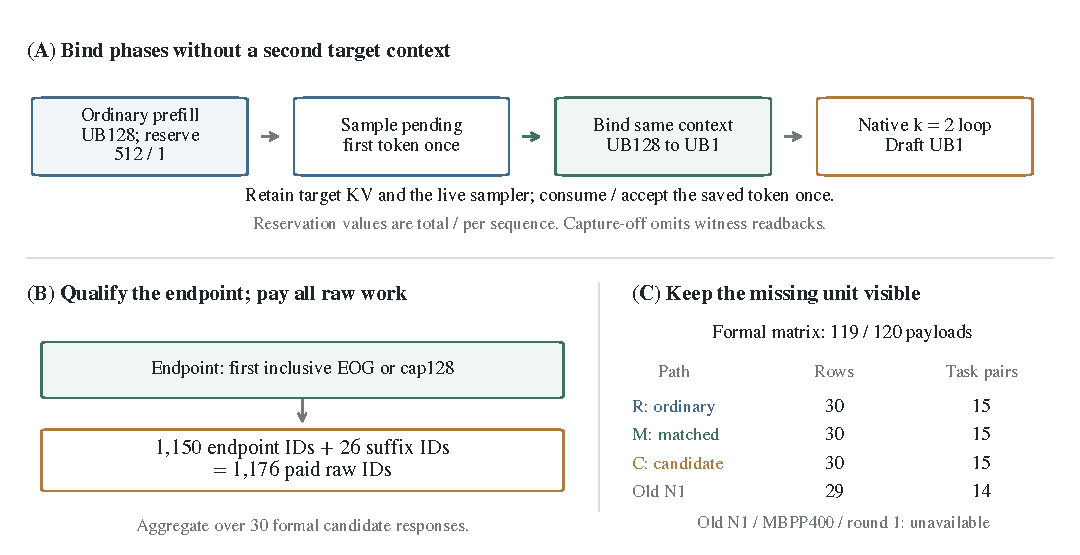
\includegraphics[width=\linewidth]{figures/figure_S1_b570_contract.pdf}
\caption{B570 implementation and accounting boundaries. (A) Ordinary prefill, one pending sample, in-place phase binding and the native loop retain one target context and live sampler; this is a source-bound schematic, not a timing profile. Reservation values are total/per sequence. (B) The endpoint gate retains IDs through the first inclusive EOG or cap128, while all online suffix work remains paid. The counts aggregate 30 formal candidate responses. (C) Available payloads and complete two-round task pairs remain distinct; the missing old-N1 MBPP/400 round-1 payload is unavailable, not zero cost.}
\label{fig:b570_contract}
\end{figure*}
% REVISION_ADDITION_END

\subsection{Qualification counts and unresolved raw comparisons}
\label{supp:b570_missingness}
Table~\ref{tab:b570_qualification} reports endpoint and raw-array comparisons separately. The 48 baseline-development rows have only 32 ordinary-reference-equal endpoints; they are not all qualified candidate evidence. The 12 shams are separate from the 299 rows in the qualification export. Stage D contains 56 exposed tasks evaluated twice. Stage E combines eight bridge records and 119 formal records; their roles are not interchangeable.

\begin{table*}[t]\centering\small
\caption{B570 candidate qualification stages and raw comparison limits. Equality is to the registered endpoint reference unless stated otherwise.}
\label{tab:b570_qualification}
\begin{tabularx}{\linewidth}{@{}>{\raggedright\arraybackslash}p{.25\linewidth}rr>{\raggedright\arraybackslash}X@{}}\toprule
Stage & \shortstack{Candidate\\checks} & \shortstack{Endpoint\\equal} & Raw reference comparison\\\midrule
C development & 12 & 12 & Four equal, eight different\\
D exposed bridge & 112 & 112 & MBPP: 16 equal/48 different; 48 HumanEval raw comparisons unknown\\
E candidate formal & 30 & 30 & Included in the E total below; suffix cost retained\\
E all available plus bridge & 127 & 127 & 80 equal, 47 different\\\bottomrule
\end{tabularx}
\end{table*}

The four-condition formal matrix is 119/120. The missing unit is \nolinkurl{E/FORMAL/1/old_N1/MBPP/400}, with \nolinkurl{INFRASTRUCTURE_INTERRUPTION_NO_PAYLOAD}. Its runtime cost and interrupted teardown time remain unknown. Each of ordinary $R$, matched $M$ and candidate $C$ has 30 complete formal observations and 15 complete two-round task pairs. Old N1 has 29 observations and only 14 complete task pairs. The available MBPP/400 old-N1 round is retained but cannot supply its two-round median. There is no interpolation, zero-cost assumption, silent task removal from other comparisons or scientific rerun. The study's administrative closeout remains \nolinkurl{PARTIAL_INFRASTRUCTURE_BUDGET_CLOSED}.

\subsection{All measured timers and work}
\label{supp:b570_costs}
Generation time is the frontend's registered C++ interval, including pending-state initialization, sampler/batch operations, phase binding within that interval, draft/verification, rollback and final synchronization. Whole-request time also includes prefill/reset/cleanup, excluding subsequent disk file writes. Host request time is separately measured by Windows QPC. Earlier A/B stage GetTickCount's 15.625-ms granularity is not substituted for formal C/D/E QPC measurements. Model-load cost is outside these comparisons.

The main manuscript's B570 paid-cost table reports all three formal timer aggregates. Table~\ref{tab:b570_task_cost} provides all paired task generation and whole-request ratios. R/C and M/C are below one on every complete task and round. Old-N1/C whole and host request ratios reverse on MBPP/245 in round 2, approximately 0.873582 and 0.873603; aggregate old-path improvement therefore does not imply universal improvement.

% Generated by scripts/reconstruct.py from frozen exports.
\begingroup\small
\begin{table*}[t]\centering
\caption{All B570 two-round task-median speed ratios. G/W denote generation/whole request; old N1 has no complete pair for MBPP/400.}\label{tab:b570_task_cost}
\begin{tabular}{@{}rrrrrrr@{}}
\toprule
MBPP & $R/C$ G & $R/C$ W & $M/C$ G & $M/C$ W & N1/$C$ G & N1/$C$ W\\\midrule
125 & 0.320296 & 0.270051 & 0.319891 & 0.243047 & 2.437945 & 1.908679\\
130 & 0.299904 & 0.252594 & 0.304551 & 0.257891 & 2.269168 & 1.978931\\
132 & 0.264679 & 0.162455 & 0.271252 & 0.169635 & 8.515349 & 4.089033\\
245 & 0.298694 & 0.254655 & 0.298448 & 0.255268 & 1.541642 & 1.376354\\
278 & 0.270026 & 0.205714 & 0.271973 & 0.245382 & 3.078819 & 2.321202\\
312 & 0.257757 & 0.195314 & 0.259093 & 0.198785 & 4.282380 & 2.984986\\
400 & 0.265906 & 0.153521 & 0.269833 & 0.158972 & -- & --\\
429 & 0.276956 & 0.197973 & 0.281509 & 0.203527 & 3.441493 & 2.411608\\
435 & 0.260099 & 0.151096 & 0.266645 & 0.158111 & 6.873734 & 3.323427\\
446 & 0.305206 & 0.233673 & 0.306943 & 0.272100 & 2.479117 & 1.929448\\
451 & 0.273297 & 0.193117 & 0.276409 & 0.198226 & 4.774253 & 3.079460\\
470 & 0.281105 & 0.243139 & 0.284055 & 0.199636 & 4.389394 & 2.870175\\
475 & 0.276814 & 0.196772 & 0.278850 & 0.201003 & 5.011890 & 3.193580\\
479 & 0.310439 & 0.196746 & 0.312663 & 0.200719 & 5.061865 & 2.965935\\
69 & 0.286855 & 0.163151 & 0.292541 & 0.169808 & 8.776569 & 4.056630\\
\bottomrule\end{tabular}
\end{table*}

\endgroup


Candidate formal endpoint IDs total 1,150 and raw IDs 1,176. All 26 suffix IDs are charged. Drafted/accepted IDs total 888/702, and target/draft continuation caller tokens 1,332/1,362. These denominators describe different runtime quantities and cannot be collapsed into one acceptance-adjusted cost. The narrowed target common-sampling measurement of 851.52 ms omits other work; it is not a full component profile. The known complete-campaign host subtotal is approximately 6,541.86 s, excluding the unknown interruption/teardown. It is not the cost of every planned request or a normalized per-task speed estimator.


\section{Historical Costs, Stops, Control, and Target-Work Budgets}
\label{supp:history}
\subsection{Early four-system inventory and unchanged estimators}
\label{supp:historical_inventory}
The historical inventory uses MacBook Air M4/Metal (llama.cpp b10809), Core Ultra 9 275HX plus RTX 5070 Ti Laptop/CUDA (b10839), Core i5-13400 plus Arc B570/Vulkan0 (b10839), and Core Ultra X7 358H plus Arc B390/Vulkan0 with an OpenVINO draft. Qwen3-8B Q8\_0 is the target. Draft is Qwen3-0.6B Q8\_0 except the symmetric INT4 OpenVINO adapter. Hardware, OS, backend, placement and frontend vary jointly. The inventory is not a hardware-only comparison or a common energy/latency ranking.

Table~\ref{tab:historical_cost} reports the completed historical campaigns. M4's representative 24Q and separately preregistered HumanEval30 have opposite measured outcomes in distinct sessions. This does not identify a workload-only cause. Early MLX precision/correctness failures are separate from the final Q8\_0 Metal configuration. RTX historical CPU-to-GPU and same-GPU controls retain different integration costs. B570's formal failure triggers its stop; a later six-prompt serial text probe passes 18/18, whereas its full 30-prompt serial text comparison reaches only 60/90. Remote-interaction-contaminated diagnostic observations are excluded from the final cells. Legacy ``exact'' labels do not upgrade the text contract.

\begin{table*}[t]\centering\small
\caption{Historical latency outcomes under their original contracts. Intervals are descriptive and source-specific. Text agreement is not a direct-ID certificate.}
\label{tab:historical_cost}
\begin{tabularx}{\linewidth}{@{}Xrrl@{}}\toprule
Campaign & Speed & Interval & Agreement\\\midrule
M4 representative 24Q & 0.842 & [0.809,0.877] & 72/72 text\\
M4 HumanEval30 & 1.387 & [1.351,1.422] & 90/90 text\\
RTX CPU draft, HumanEval30 & 0.404 & [0.390,0.418] & 90/90 text\\
RTX same-GPU draft, HumanEval30 & 0.650 & [0.629,0.673] & 90/90 text\\
B570 serialized fallback & 0.3087 & [0.2927,0.3246] & 60/90 text\\
358H CPU stateful, HumanEval30 & 0.733915 & [0.692920,0.771090] & 90/90 IDs\\
358H NPU stateful, HumanEval30 & 0.351663 & [0.332595,0.368949] & 90/90 IDs\\\bottomrule
\end{tabularx}
\end{table*}

Historical M4 24Q takes a within-prompt GM of three paired ratios, then resamples prompts 10,000 times with Python Random seed 20260907 and sorted draw indices 249/9749. M4 HumanEval uses the same within-prompt aggregation but 100,000 draws, seed 20260910 and indices 2500/97499. Historical RTX uses 10,000 draws, seed 20260910, indices 249/9749. B570 fallback uses 10,000 draws, seed 20260910 and indices 250/9750 in archived insertion order. Sorting tasks changes its finite-seed endpoints and is not substituted. 358H uses prompt medians of three paired ratios, 10,000 draws, NumPy default\_rng seed 20260919 and .025/.975 quantiles. These policies are not replaced by late RTX's ratio-of-medians estimator.

\subsection{Target-forward proxies and energy boundaries}
\label{supp:historical_proxies_energy}
The historical target-only proxy is
\[
V_k^{\mathrm{micro}}(n,e)=T_{\mathrm{target\ forward}}(k,n,e)/T_{\mathrm{target\ decode}}(1,n).
\]
It omits drafting and can omit correction/bonus, state work and complete target-round bookkeeping. Table~\ref{tab:proxy_lookup} retains every context cell. Their ranges span contexts rather than uncertainty intervals. The historical RTX HumanEval/106 diagnostic repeats a same-position argmax change from 2790 to 2629 three times, with a separately instrumented same-commit margin moving from $+0.080948$ to $-0.126457$. It is shape-sensitive evidence in that configuration, not a unique kernel cause or a formal timing observation.

\begin{table}[ht]\centering\small
\caption{Frozen target-forward proxy lookup. These are neither complete target-round cost nor integrated speed. Historical text agreement applies only under each original comparator.}
\label{tab:proxy_lookup}
\begin{tabular}{@{}lrr@{}}\toprule
Path & Context & $V_2^{\mathrm{micro}}$\\\midrule
M4 Metal & 512 & 1.022182\\
M4 Metal & 2048 & 1.076126\\
M4 Metal & 8192 & 1.032264\\
RTX batched & 0 & 1.009030\\
RTX batched & 256 & 0.983148\\
RTX serialized & 0 & 2.430996\\
RTX serialized & 256 & 2.137011\\
B570 fast & 512 & 1.242576\\
B570 fast & 2048 & 1.637295\\
B570 serialized & 512 & 1.982668\\
B570 serialized & 2048 & 1.991707\\\bottomrule
\end{tabular}
\end{table}

M4 HumanEval energy measures the Silemetry CPU+GPU+ANE package aggregate, excluding separate DRAM. Fixed-$k=2$ package efficiency is $1.013\times$ with interval $[0.990,1.034]$, so improvement is not established. The registered secondary $p_{\min}=0.9$ condition has $1.041\times$ $[1.018,1.065]$, without replacing the primary or establishing material added speed. The corrected synthetic ceiling was registered but not executed; earlier synthetic diagnostics are not a substitute.

RTX board and CPU-package sensors are distinct domains, and follow-up process windows include loading; no formal serial HumanEval energy comparison is claimed. B570 fallback measures adapter-board efficiency $0.302\times$ $[0.285,0.320]$, without CPU package or wall power, and its output failure confines the result to diagnosis. 358H has no qualified end-to-end energy boundary. No late runtime repair energy, common system-energy ranking or concurrent-throughput result is inferred.

\subsection{Fresh direct-ID gates and independent latency arm}
\label{supp:historical_id_gates}
Fresh RTX direct-ID v2 has 270 executions on 30 HumanEval tasks, three conditions and three repeats. Batched $k=2$ reaches 75/90 (25/30 wholly equal prompts) and is blocked; serialized reaches 90/90 and qualifies. Mismatching first indices are /64:114, /106:65, /119:17, /128:41 and /129:21, stable across repeats. All conditions repeat stably. The initial v1 transport study retains 83 executions, 82 valid, and no qualification result: full-log UTF-8 decoding fails on a partial draft fragment after native exit zero. V2 changes observational byte transport and restarts the whole frozen schedule; it imports no v1 formal pairs. The final report stored at the repository's v1 path is a copy of the completed v2 report; it does not document v1 completion.

B570's separate fresh direct-ID campaign also completes 270 executions: fast reaches 60/90 (20/30 prompts), serialized 78/90 (26/30), and both are blocked. Historical fast 45/90 and serial 60/90 are unchanged text-path counts. An initial metadata decoding launch fails before inference with zero formal executions; authorized direct execution of the unchanged frozen runner produces the full campaign. No formal speed is inferred from operational elapsed fields. Neither new gate retroactively qualifies old timings.

The independent RTX matched-latency arm has 180 fresh timing observations and 90/90 fresh complete-ID agreements on 30 tasks. Serialized speed is $0.645816\times$, interval $[0.629802,0.659884]$, zero of 30 faster. Condition order uses seed 2026093001; the 10,000 prompt-bootstrap draws use seed 2026093002 and linear percentiles. Native QPC timing starts after synchronized target/draft prefill and covers per-request sampler/state work, drafting, verification, acceptance/correction/bonus, rollback, synchronization, logging/response and slot release. Load and teardown are excluded. Chrono shares the host oscillator; it is not an independent physical clock. The empty-hook probe bounds clock-call overhead, not all logging overhead. The fresh frontend is compiled with Clang 21.1.0 over retained CUDA libraries; OS build 26300 differs from the earlier direct-ID OS26200. These facts preclude synthetic pairing with prior qualification.

\subsection{V3 stop, V4 recovery, and protocol amendment}
\label{supp:v3_v4}
V3 plans 576 formal condition/repetition rows over 24 tasks. It delivers 126 valid prefix rows: 72 pre-live and 54 cost, with two failures and 448 unreached rows. Native HumanEval/59 emits 128 committed IDs ending at EOG and reports both limit and EOS. The frozen parser accepts only one marker and stops. Exit zero is not sufficient to make capture valid. A-live receives zero formal runs; complete formal accuracy, speed and interval are unavailable. Engineering qualification's 400 runs and parser-negative fixtures do not repair the missing formal endpoint branch. Old failures remain sealed.

V4 fixes that observational endpoint handling under a new freeze, accepting the ordered complete EOS-at-cap case while rejecting contradictory, reversed, duplicate or missing markers. Its 19-task panel initially comprises the remaining project-unused HumanEval inputs; subsequent reuse is exposed. It retains 228 pre-live predictor records and adds 57 native live and 171 fresh timing observations: 456 complete formal condition rows. Prediction closure is described in Section~\ref{supp:diagnosis}. The cost arm uses one timer executable and balanced order, each condition appearing in each order position 19 times. Batched qualification remains 51/57 and has no admissible speed/interval. Global serialization qualifies 57/57 but yields $0.677351\times$ $[0.661653,0.691812]$, zero of 19 faster. Median task absolute times are 1.607 s target and 2.332 s serial; their ratio is not the paired GM. The interval uses 10,000 paired-row draws, seed 2026100204 and linear quantiles.

The V4 numerical sources and assets remain frozen, but a fan-curve change triggers the original strict host-hash stop before live outcomes. Authorized continuation preserves the original \texttt{PROVENANCE\_INVALID} records, repeated predictor checks and the amendment. Fan/lighting differences become permitted; non-fan material settings remain strict. Predictor data are reused, not relabeled as a fresh untouched cohort. Fan controls stay fixed during the fresh timing arm, with snapshots retained, but can still affect latency. The campaign completed under the disclosed amendment; the original no-deviation host policy did not pass. Instrumented post-prefill-to-slot-release time is distinct from the later server generation field and cannot form a common optimization curve.

\subsection{RTX efficiency screening}
\label{supp:rtx_efficiency_pilot}
The early FA-on/UB512 four-probe pilot qualifies small-model $k=2$ and $k=4$, with request/generation speeds $1.277\times/1.324\times$ and $1.492\times/1.572\times$. Each FA/UB setting has its own ordinary reference; global UB changes several phases. Expansion to HumanEval/0--7 preserves every failure: final small-model $k=2$ qualifies 18/24, fragment drafting 21/24 and the mixed strategy 15/24. A mixed result producing 18 rather than the reference 87 IDs is invalid as a speed claim. $k=2$ repairs /5 but introduces /2; /6 remains divergent. The campaign has 300 formal requests and 48 excluded warmups. Synthetic favorable cases do not support the current headline.

\subsection{M4 formal control and oracle opportunity}
\label{supp:m4_control}
The M4 Guard measures cumulative charged generation time per committed ID, including seed/correction/bonus and excluding rejected proposals. It starts on Always speculation and can fall back permanently after a completed round, reconciling invalid target/draft suffixes first. Calibration freezes target cost per ID and selects \texttt{E8\_M000} from a nine-candidate grid with rounds $\{2,4,8\}$ and margins $\{0,0.05,0.10\}$. Exactness and calibration regret select the rule; ties use frozen overhead/exploration/margin/ID rules. Disjoint calibration, qualification and held-out task IDs prevent held-out retuning. Online decisions receive no future length, task family, request-specific target latency or oracle answer.

The registered post-prefill clock includes generation initialization, seed sampling, draft/target work, synchronization, reconciliation, control and transition. Load, sampler/speculator setup, initial prefill and the speculative begin hook precede it. This is not whole HTTP request latency. The formal campaign has 60 held-out tasks, 30 each HumanEval and Spec-Bench, three conditions and three repeats. Always and Guard each qualify 180/180 IDs. Table~\ref{tab:m4_strata} gives their original overall and family estimates.

% Generated by scripts/reconstruct.py from frozen exports.
\begin{table*}[t]\centering\small
\caption{M4 formal post-prefill baseline/candidate speeds from three-repeat condition medians. Family strata are descriptive.}\label{tab:m4_strata}
\begin{tabular}{@{}lrrr@{}}\toprule
Panel & Tasks & Target/Always & Target/Guard\\\midrule
Overall & 60 & 1.346894 & 1.311387\\
HumanEval & 30 & 1.570011 & 1.554690\\
Spec-Bench & 30 & 1.155485 & 1.106160\\
\bottomrule\end{tabular}

\end{table*}


The primary 10,000-draw bootstrap uses Python Random seed 20260924 in held-out order, with one continued stream for target/Guard, target/Always and Guard/oracle. The paired Guard/Always secondary replay starts a fresh stream of the same seed and uses linear percentiles; it gives latency $1.027076$ $[1.012956,1.043559]$, with Guard faster on 24 and Always on 36 tasks. It is post-study, not the original preregistered endpoint. A separate family-stratified sensitivity uses seed 2026100101, 10,000 draws and HumanEval-then-Spec-Bench order, giving $[1.0135,1.0423]$; it leaves the original intervals unchanged.

The per-task two-fixed-mode oracle improves the measured interval by factor $1.0006919671$ relative to Always. The implied latency reduction is $1-1/1.0006919671=0.0006914886$, approximately 0.069149\%. Only Spec-Bench/559 and /95 favor target-only: target times are 11.9085 and 10.9203 s; Always/target latencies 1.0270 and 1.0150; Guard/target 1.0215 and 1.0029. This finite hindsight opportunity is not a bound on all intra-request policies.

A loop-variable shadowing defect records a build-manifest digest in the intended calibration-freeze field. Recovery verifies the actual freeze, source/model/calibration/policy hashes and formal-start links, retaining error markers and the original pipeline \texttt{STOPPED} metadata. It does not retune the policy or mutate measurements. Recorded Git order is not a trusted external timestamp. The resolved metadata defect does not change the formal experiment's completion status.

\subsection{358H state interface, threshold gate, and conditional budgets}
\label{supp:358h_budgets}
The 358H stateful runner is complete; the preceding preflight scaffold was empty and blocked. It keeps the target's low-level context between rounds and charges validation, rejected-suffix rollback, correction/bonus and synchronization within complete target work. Every OpenVINO proposal call receives the full committed prefix. The synchronous region combines replay/reconstruction and proposal, with no separate measurements of those terms.

A prior proxy threshold study passes 18 direct-ID sanity pairs and admits borderline context points, using a favorable zero residual $T_x$, fixed progress assumptions and seed 20260919, 10,000 empirical draws. It predicts eligibility, not achieved integrated speed. CPU central/optimistic speeds at contexts512/2048/8192 are 0.903680/1.355520, 0.884843/1.327264 and 0.755946/1.133919. NPU values are 0.905553/1.358329, 0.903804/1.355706 and 0.839618/1.259427. The subsequent actual stateful CPU/NPU speeds in Table~\ref{tab:historical_cost} are lower and qualified, with zero of 30 prompts faster on either path.

Table~\ref{tab:358h_accounting} retains measured progress, components and distinct ceiling estimators. Both paths commit 11,520 IDs, over 4,677 CPU and 4,686 NPU rounds. Arithmetic-total accounting gives normalized $(D,R,X)=(0.4304,2.9767,0.00124)$ CPU and $(4.1251,2.9435,0.00130)$ NPU. These values reproduce total-time ratios, not prompt GMs. Target-only ceilings assume unchanged baseline, target work and progress with all other nonnegative cost removed.

Let $B_{ij}$ be matched target-only time and $T_{ij}$ measured complete target work for prompt $i$ and repetition $j$. If optimized speculative time retains this target work and only reduces the other nonnegative costs, its speed $S'_{ij}$ is at most $B_{ij}/T_{ij}$. Monotonicity of the median and geometric mean then gives the bound under the original prompt estimator:
\begin{equation}
\operatorname{GM}_{i}\operatorname{median}_{j} S'_{ij}
\leq \operatorname{GM}_{i}\operatorname{median}_{j}(B_{ij}/T_{ij}).
\label{eq:floor}
\end{equation}
For a uniform fractional reduction $\delta$ in target work, the corresponding zero-other-work ceiling increases by $1/(1-\delta)$. If its original value is $F<1$, parity therefore requires $\delta\geq 1-F$. Table~\ref{tab:358h_accounting} reports this necessary budget separately for the prompt and pooled-total estimators. It assumes fixed baseline and committed progress; changing either requires fresh qualification and measurement.

% REVISION_ADDITION_BEGIN: 358H conditional budget visual explanation
Figure~\ref{fig:358h_budget} places the measured prompt-estimator speeds beside their conditional ceilings and the necessary target-work cuts. The pooled-total estimator remains separate in Table~\ref{tab:358h_accounting}.

\begin{figure*}[t]
\centering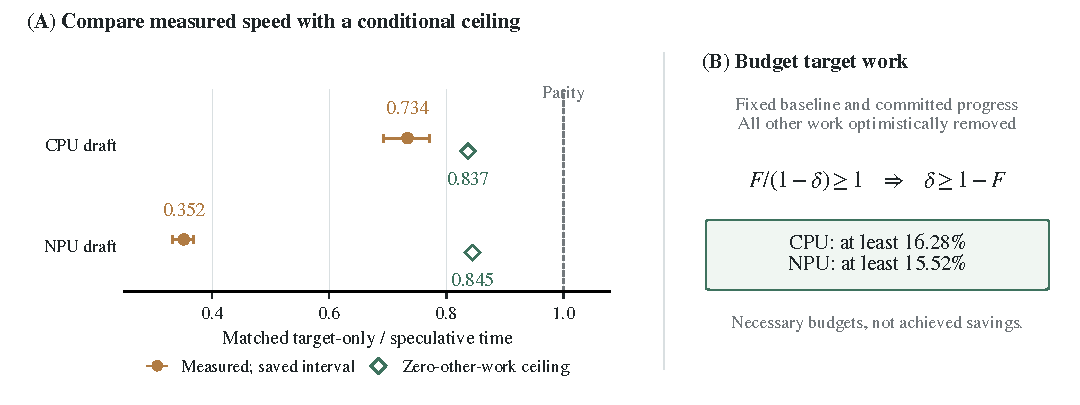
\includegraphics[width=\linewidth]{figures/figure_S2_358h_budget.pdf}
\caption{358H measured speed and a conditional optimization budget. (A) Filled circles and bars show the saved speed estimates and descriptive prompt-bootstrap intervals; open diamonds show arithmetic ceilings if all other nonnegative work were removed while baseline, target work and committed progress stayed fixed. All points use the original geometric mean of 30 prompt medians of three paired ratios. Ceiling markers have no confidence intervals. (B) Reaching parity in that optimistic case requires a uniform target-work cut of at least $1-F$, where $F$ is the original ceiling. These are necessary budgets, not achieved savings or an impossibility claim about NPUs. The 180-row original-host ceiling audit remains inherited.}
\label{fig:358h_budget}
\end{figure*}
% REVISION_ADDITION_END

\begin{table*}[t]\centering\small
\caption{358H measured accounting and conditional zero-other-work ceilings. Percentages describe the saved synchronous regions; prompt and pooled estimators remain distinct.}
\label{tab:358h_accounting}
\begin{tabular}{@{}lrr@{}}\toprule
Quantity & CPU draft & NPU draft\\\midrule
Committed IDs per round & 2.463117 & 2.458387\\
Replay plus proposal share (\%) & 12.6273 & 58.3474\\
Complete target-work share (\%) & 87.3365 & 41.6342\\
Residual share (\%) & 0.0363 & 0.0184\\
Actual pooled-total speed & 0.7227 & 0.3477\\
Pooled-total ceiling & 0.8274529834 & 0.8351858524\\
Prompt-estimator ceiling & 0.8372192092 & 0.8448401086\\
Necessary uniform target cut, prompt (\%) & 16.278079 & 15.515989\\
Necessary uniform target cut, pooled (\%) & 17.254702 & 16.481415\\\bottomrule
\end{tabular}
\end{table*}

No prompt-median ceiling reaches parity; maximum prompt ceilings are 0.9736196764 CPU and 0.9999089575 NPU. One NPU repetition has $B/T=1.000163695$, so not every individual run-level ceiling is below one. The budgets are necessary arithmetic reductions under fixed progress, not achieved optimizations or proof against NPUs. A persistent-state/wider-target candidate stops at qualification: CPU restore/reconcile correctness is unavailable under the tested representation, and the frozen dynamic-shape NPU IR lacks the required state-capable path. Same-prefix target-only and proposal-replay diagnostics identify greedy divergence but not a unique rollback bug. No formal runtime performance or energy result exists for that failed candidate; the completed earlier Phase-3 costs remain valid under their own contract.


\section{CPU Reconstruction, Provenance, and Access Limits}
\label{supp:reproducibility}
The author source package contains editable LaTeX, vector PDF/SVG figures, bibliography, Highlights, CPU verification and build scripts, selected authenticated implementation/report records, the 26-claim evidence map and the 28-group experiment ledger. Compile \texttt{main.tex} or \texttt{supplement.tex} with pdfLaTeX using the supplied assets. The build scripts recheck frozen exports. The figures express categorical relationships and consistent comparison roles while retaining the bound observations, numerical values and intervals. Two supplementary figures explain the bound B570 source/exports and 358H saved estimates/budgets. The double-column supplement includes every inherited table cell and result. Structured and flat source archives are separately rebuilt; compilation does not establish live Overleaf or Editorial Manager acceptance.

The verifiers authenticate the copied-source bindings and reconstruct the RTX 384-row matrix, response-ID digest joins, qualification flags, absolute-time medians, all 12 cost comparisons, descriptive intervals, task regressions, round reversal and ratio identities. They reconstruct B570's 119 formal rows, 15 versus 14 complete task pairs, three timers and paid suffix counts. Phase booleans, natural-cross matrices, fixed-UB task-ratio aggregates and M4 medians/oracle are also checked. Version-specific receipts identify the source, figure, PDF and archive hashes actually checked; earlier receipts retain their historical attribution.

These checks operate on included sources and compact exports. The original runtime reports retain original-host audits, external-asset hashes and references to larger private archives. Those audits are inherited evidence: the current checks neither reopen every raw payload nor rehash omitted model/driver binaries, validate independent absolute timing or rerun inference. Reproducing a summary or task-ratio export is not a complete raw-data audit. The missing B570 payload, interruption cost and unknown historical raw comparisons remain unresolved.

Dataset and software descriptions are cited in the main manuscript~\cite{humaneval,mbpp,specbench,llamacpp,qwen3}. Bibliographic versions and pending metadata checks are documented in the author records. Authorship, affiliations, CRediT, funding, competing interests, permissions, permanent data/software access and the final AI-assistance statement require author confirmation. A second model family, same-contract external method comparisons, stochastic sampling and concurrent throughput are outside the completed evidence scope.

\FloatBarrier
\begingroup\small
\bibliographystyle{elsarticle-num}\bibliography{references}
\endgroup
\end{document}
